%\chapter{Theoretical Background}
%\framebox{REVIEW1}
\section{A Brief Introduction to SVM-HMM}
\label{sec:svm-hmm}
In this thesis, we use structural support vector machine to learn performance knowledge from expressive performance samples. Unlike traditional SVM algorithm, which can only produce univariate prediction, structural SVM can produce structural predictions like tree, sequence and hidden Markov model. Structural SVM with hidden Markov model output (SVM-HMM) has been successfully applied to part-of-speech tagging problem\cite{svm2009}. The part-of-speech tagging problem has some similarity with expressive performance problem. In part-of-speech tagging, one tries to identify the role by which the word plays in the sentence, while in expressive performance, one tries to determine how a note should be played, usually based on it's role in the musical phrase. For example, an authentic cadence at the end of a phrase is usually played louder and stronger than a embellishment note in the middle of a phrase. Thus, we believe SVM-HMM will be a good candidate for expressive performance. The following introduction and formulas relies heavily on \cite{svm2009, svm2005, svm2003}.

%Ref: 20130420 slides

%TODO:discuss traditional SVM here?
Traditional SVM prediction problem can be described as finding a function 
$$h: \mathcal{X \rightarrow Y}$$ with lowest prediction error. $\mathcal{X}$ is the input features space, and $\mathcal{Y}$ is the prediction space. In traditional SVM, elements in $\mathcal{Y}$ are labels (classification) or real values (regression). But structural SVM extends the framework to generate structural output, such as tree, sequence, or hidden Markov model.
To extend SVM to support structured output, the problem is modified as finding a discriminant function $f: \mathcal{X} \times \mathcal{Y} \rightarrow \mathcal{R}$, in which the input/output pairs are mapped to a real number score. To predict an output $y$ for an input $x$, one try to maximize $f$ over all $y \in \mathcal{Y}$. 

$$h_{\mathbf{w}}(x) = \argmax_{y\in\mathcal{Y}} f_{\mathbf{w}}(x,y)$$

Let $f_{\mathbf{w}}$ be a linear function of the form:

$$ f_{\mathbf{w}} = \mathbf{w}^{T}\Psi(x,y)$$, 
where $\mathbf{w}$ is the parameter vector, and $\Psi(x,y)$ is the kernel function relating input $x$ to output $y$. $\Psi$ can be defined to accommodate various kind of structures. 

%emprical risk
For each structure we want to predict, a loss function that measures the accuracy of of a prediction is required. A loss function $\Delta:\mathcal{Y}\times\mathcal{Y}\rightarrow R$ need to satisfy the following property:

$$\Delta(y, y') \geq for\ y \neq y'$$
$$\Delta(y, y) = 0 $$

The loss function is assumed to be bounded. Let's assume the input-output pair $(x,y)$ is drawn from a join distribution P(x,y), the prediction problem is to minimize the total loss:

%TODO: total loss formula 2005 sec 2.1
$$R_p^\Delta = \int_{\mathcal{X} \times \mathcal{Y}} \Delta (y, f(x))dP(x,y)$$

Since we can't directly find the distribution $P$, we need to replace this total loss with a empirical loss, which can be calculated from the observed training set of $(x_i, y_i)$ pairs.
%TODO: emprical loss
$$R_s^\Delta(f) = \frac{1}{n}\sum^n_{i=1}\Delta(y_i, f(x_i))$$

Now we are ready to extend SVM to structural output, starting with a linear separable case, and we will then extend it to soft-margin formulation. 

A linear separable case can be expressed by a set of linear constrains
%TODO: 2005 formula 4
$$\forall i \in \{1,\cdots,n\}, \forall \hat{y_i}\in\mathcal{Y}: \mathbf{w}^T [\Psi(x_i, y_i) - \Psi(x_i, \hat{y_i})]\leq 0$$

However, in the SVM context, we want the solution to have the largest margin possible. So the above linear constrains will become this optimization problem:
%TODO: 2005 formula 4+
$$
\begin{aligned}
& \max_{\gamma, \mathbf{w}:\|\mathbf{w}\| = 1} \gamma \\
& s.t \; \forall i \in \{1,\cdots,n\}, \forall \hat{y_i} \in\mathcal{Y}: \mathbf{w}^T [\Psi(x_i, y_i) - \Psi(x_i, \hat{y_i})] \leq \gamma\\
\end{aligned}
$$

, which is equivalent to the convex quadratic programming problem:
%TODO: 2005 formula 5,k 6
$$
\begin{aligned}
   & \min_{\mathbf{w}, \xi_i \geq 0} \frac{1}{2}\mathbf{w}^T\mathbf{w} \\\
    &s.t.\; \forall i \in \{1,\cdots,n\},\hat{y_i} \in \mathcal{Y}: \mathbf{w}^T[\Psi(x_i,y_i) - \Psi(x_i,\hat{y_i})] \geq 1\\
\end{aligned}
$$

To extend the linear-separable case to non-separable case, slack variables $\varepsilon_i$ can be introduced to penalize prediction errors, results in a soft-margin formalization:
%TODO: 2005 formula SVM1
$$
\begin{aligned}
   & \min_{\mathbf{w}, \xi_i \geq 0} \frac{1}{2}\mathbf{w}^T\mathbf{w} + \frac{C}{n}\sum^n_{i=1}\xi_i\\
    &s.t.\; \forall i \in \{1,\cdots,n\},\hat{y_i} \in \mathcal{Y}: \mathbf{w}^T[\Psi(x_i,y_i) - \Psi(x_i,\hat{y_i})] \geq 1 - \xi_i \\
\end{aligned}
$$

$C$ is the weighting parameter controlling the trade-off between low training error and large margin. The optimal $C$ varies between different problems, so experiment should be conducted to find the optimal $C$ for our problem.

Intuitively, a constrain violation with larger loss should be penalize more than the one with smaller loss. So I. Tsochantaridis et al. \cite{svm2005} proposed two possible way to take the loss function into account. The first way is to re-scale the slack variable by the inverse of the loss, so a high loss leads to smaller re-scaled slack variable:
%slack rescaling

$$
\begin{aligned}
   & \min_{\mathbf{w}, \xi_i \geq 0} \frac{1}{2}\mathbf{w}^T\mathbf{w} + \frac{C}{n} \sum^n_{i=1}\xi_i\\
    &s.t.\; \forall i \in \{1,\cdots,n\},\hat{y_i} \in \mathcal{Y}: \mathbf{w}^T[\Psi(x_i,y_i) - \Psi(x_i,\hat{y_i})] \geq 1 - \frac{\xi_i}{\Delta(y_i, \hat{y_i})} \\
\end{aligned}
$$

The second way is to re-scale the margin, which yields 
%margin-rescaling
$$
\begin{aligned}
   & \min_{\mathbf{w}, \xi_i \geq 0} \frac{1}{2}\mathbf{w}^T\mathbf{w} + \frac{C}{n} \sum^n_{i=1}\xi_i\\
    &s.t.\; \forall i \in \{1,\cdots,n\},\hat{y_i} \in \mathcal{Y}: \mathbf{w}^T[\Psi(x_i,y_i) - \Psi(x_i,\hat{y_i})] \geq \Delta(y_i, \hat{y_i}) - \xi_i\\
%
\end{aligned}
$$

But the above quadratic programming problem has a very large number ($O(n|\mathcal{Y}|)$) of constrains , which will take considerable time to solve. I. Tsochantaridis et al. \cite{svm2005} proposed a greedy algorithm to speed up the process by selecting only part of the constrains that contributes the most to finding the solution. Initially, the solver starts with an empty working set containing no constrains. Than the solver iteratively scans the training set to find the most violated constrains under the current solution. If a constrain is violated more times than a desired threshold, the constrain is added to the working set of constrains. Then the solver re-calculate the solution under the new working set. The algorithm will terminate once no more constrain can be added under the desired precision.

In a later work by Joachims et al.\cite{svm2009}, they created a new formulation and algorithm to further speed up the algorithm. Instead of using one slack variables for each training sample, which results in a total of $n$ slack variables, they use a single slack variable for all $n$ training samples. The following formula is the 1-slack version of slack-rescaling structural SVM:
%1-slack
$$
\begin{aligned}
    & \min_{\mathbf{w}, \xi_i \geq 0} \frac{1}{2}\mathbf{w}^T\mathbf{w} + C \xi\\
    &s.t.\; \forall i \in \{1,\cdots,n\},\hat{y_i} \in \mathcal{Y}: \mathbf{w}^T[\Psi(x_i,y_i) - \Psi(x_i,\hat{y_i})] \geq \frac{1}{n}\sum^n_{i=1}1 - \frac{\xi}{\Delta(y_i, \hat{y_i})} \\
\end{aligned}
$$

And margin-rescaling structural SVM:

$$
\begin{aligned}
    & \min_{\mathbf{w}, \xi_i \geq 0} \frac{1}{2}\mathbf{w}^T\mathbf{w} + C \xi\\
    & s.t.\; \forall i \in \{1,\cdots,n\},\hat{y_i} \in \mathcal{Y}: \mathbf{w}^T[\Psi(x_i,y_i) - \Psi(x_i,\hat{y_i})] \geq \frac{1}{n}\sum^n_{i=1}\Delta(y_i, \hat{y_i}) - \xi \\
\end{aligned}
$$
%                $$\min_{\mathbf{w}, \xi_i \geq 0} \frac{1}{2}\mathbf{w}^T\mathbf{w} + \frac{C}{n} \sum_{i=1}^{n} \xi_i$$
%                s.t. for $i = 1\cdots n$
%                $$\forall \hat{y_i} \in \mathcal{Y}: \mathbf{w}^T[\Psi(x_i,y_i) - \Psi(x_i,\hat{y_i})] \geq \Delta(y_i, \hat{y_i}) - \xi_i $$
%
%                $$\forall \hat{y_i} \in \mathcal{Y}: \mathbf{w}^T[\Psi(x_i,y_i) - \Psi(x_i,\hat{y_i})] \geq 1 - \frac{\xi+i}{\Delta(y_i, \hat{y_i})}$$
Detailed proof on how the new formulation is equally general as the old one is given in the paper \cite{svm2009}.

With the framework described above, the only problem left is how to define the general loss function for hidden Markov model (HMM)? In \cite{svm2003}, Y. Altun et al. proposed two types of features for a equal-length observation/label sequence pair $(x,y)$. The first is the interaction of a observation with a label, the other is the interaction between neighboring labels. 

%   \begin{figure*}[tp]
%      \begin{center}
%         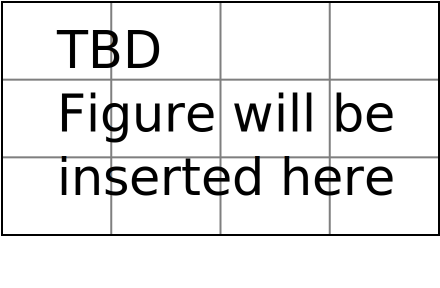
\includegraphics[width=0.8\textwidth]{fig/TBDFigure}
%      \end{center}
%      \caption{Hidden Markov Model}
%      \label{fig:hmm}
%   \end{figure*}

To illustrate the method, we use a example from music: for some observed features $\Phi_r(x^s)$ of a note $x$ located in $s$th position of the phrase, and assume $\left[ \left[ y^t = \tau \right] \right]$ denotes the $t$th note is played at a velocity of $\tau$, the interaction of the two predicate can be written as 
%TODO hmm 3 formula 4
$$\phi^{st}_{r\sigma}(\mathbf{x}, \mathbf{y}) = \left[\left[y^t = \tau \right] \right]\Psi_r(x^s),\; 1\leq\gamma\leq d,\; \tau \in \Sigma $$

And for interaction between labels, the feature can be written as
%TODO hmm 3 formula 5
$$\hat{\phi}^{st}_{r\sigma}(\mathbf{x}, \mathbf{y}) = \left[\left[y^s = \sigma \wedge y^t = \tau \right] \right],\; \sigma, \tau \in \Sigma $$

By selecting a order of dependency for the HMM model, we can further restrict $s$'s and $t$'s. For example, for a first-order HMM, $s = t$ for the first feature, and $s = t-1$ for the second feature. The two features on the same time $t$ is then stacked into a vector $\Psi(x,y;t)$. The feature map for the whole sequence is simply the sum of all the feature vectors 

%TODO hmm 3 formula 6
$$\Phi(\mathbf{x}, \mathbf{y}) = \sum^T_{t=1}\Phi(\mathbf{x}, \mathbf{y};t)$$

Finally, the distance between two feature maps depends on the number of common label segments and the inner product between the input features sequence with common labels.


$$\langle\Phi(\mathbf{x}, \mathbf{y}), \Phi(\mathbf{\hat{x}}, \mathbf{\hat{y}})\rangle = \sum_{s,t}\left[\left[y^{s-1} = \hat{y}^{t-1}\wedge y^s = \hat{y}^t\right] \right] + \sum_{s,t}\left[\left[y^{s} = \hat{y}^{t}\right] \right]k(x^s, \hat{x}^t)$$


A Viterbi-like decoding algorithm is used to speed up the computation of $F$ for HMM..


%TODO: how to define loss function for HMM?
%(2003) section 3
%ovserved output <--> tag
%previous tag <--> this tag (1-order markov)
% Psi = each note's above two property summed up
%similarity = same prev tag <--> this tag sequence + same tag <--> observed output distance

%Hard-margin one
%Soft-margin one => introduce slack variable 
%Example with large loss should be emphasized => slack rescaling
%Margin can also be scaled => margin rescaling
%There are too many constrains => greedy algo (2005), select a subset of constrains from the most violated constrains to solve
%To speed up, n-slack variables are reduced to 1-slack variable (2009)

%           \item Prediction error (risk):
%               $$R^\Delta_p(h) = \int_{\mathcal{X}\times\mathcal{Y}}\Delta(y, h(x)) dP(x,y)$$
%               \begin{tabular}{ll}
%                   where & $\Delta()$ is the loss function \footnote{Must satisfy $\Delta(x,x) = 0$, $\Delta(x,y) > 0$}\\
%                   & P(x,y) is the joint distribution of $\mathcal{X}$ and $\mathcal{Y}$
%               \end{tabular}

%    \begin{frame}{Emperical Risk}
%       \begin{itemize}
%           \item Emperical Risk from training sample $S$:\footnote{Emperical Risk Minimization Priciple (Vapnik V (1998) Statistical Learning Theory. Wiley, Chichester, GB)}

%               $$R^\Delta_S(h) = \frac{1}{n}\sum_{i=1}^{n}\Delta(y_i, h(x_i))$$
%                   where  $\Delta()$ is the loss function 

%           \item Classification SVM

%                   $$\displaystyle \min_{\mathbf{w}, \xi_i \geq 0} \frac{1}{2}\mathbf{w}^T\mathbf{w} + \frac{C}{n} \sum_{i=1}^{n} \xi_i$$
%                   s.t. $$\forall i\in {1,\cdots n}: y_i (\mathbf{w}^T x_i) \geq 1-\xi_i$$
                  

%           \item Learn a discriminant function $f:\mathcal{X} \times \mathcal{Y} \rightarrow \Re$ 
%           \item Given $x$, maximizing $f$ over all $y \in \mathcal{Y}$
%               $$h_\mathbf{w} (x) = \argmax_{y\in\mathcal{Y}} f_\mathbf{w} (x,y)$$
%           \item 
%               in which $$f_\mathbf{w} (x,y) = \mathbf{w}^T{\Psi}(x,y)$$
%               \begin{tabular}{ll}
%                   where & $\mathbf{w} \in \Re^N$ is a parameter vector\\
%                         & $\Psi(x,y)$ is a feature vector relating $x$ and $y$
%               \end{tabular}
              

 
% \section{Structural SVM}

% \section{Theoretical Details}
% %&=& &=& &=& &=& &=& &=& &=& &=& =
%    \begin{frame}{Lowest Risk}
%       \begin{itemize}
%           \item Prediction error (risk):
%               $$R^\Delta_p(h) = \int_{\mathcal{X}\times\mathcal{Y}}\Delta(y, h(x)) dP(x,y)$$
%               \begin{tabular}{ll}
%                   where & $\Delta()$ is the loss function \footnote{Must satisfy $\Delta(x,x) = 0$, $\Delta(x,y) > 0$}\\
%                   & P(x,y) is the joint distribution of $\mathcal{X}$ and $\mathcal{Y}$
%               \end{tabular}

%           %\item Training sample: $(x_1, y_1), (x_2, y_2), \cdots$ where $y_i$'s may have structural relationship
              
%       \end{itemize}
%    \end{frame}
%    \begin{frame}{Emperical Risk}
%       \begin{itemize}
%           \item Emperical Risk from training sample $S$:\footnote{Emperical Risk Minimization Priciple (Vapnik V (1998) Statistical Learning Theory. Wiley, Chichester, GB)}

%               $$R^\Delta_S(h) = \frac{1}{n}\sum_{i=1}^{n}\Delta(y_i, h(x_i))$$
%                   where  $\Delta()$ is the loss function 

%           %\item Training sample: $(x_1, y_1), (x_2, y_2), \cdots$ where $y_i$'s may have structural relationship
              
%       \end{itemize}
%    \end{frame}

%    \begin{frame}{Traditional SVM}
%       \begin{itemize}
%           \item Classification SVM

%                   $$\displaystyle \min_{\mathbf{w}, \xi_i \geq 0} \frac{1}{2}\mathbf{w}^T\mathbf{w} + \frac{C}{n} \sum_{i=1}^{n} \xi_i$$
%                   s.t. $$\forall i\in {1,\cdots n}: y_i (\mathbf{w}^T x_i) \geq 1-\xi_i$$
                  

              
%       \end{itemize}
%    \end{frame}

%    \begin{frame}{Structural SVM}
%       \begin{itemize}
%           \item Extend SVM for structural output
%           \item Learn a discriminant function $f:\mathcal{X} \times \mathcal{Y} \rightarrow \Re$ 
%           \item Given $x$, maximizing $f$ over all $y \in \mathcal{Y}$
%               $$h_\mathbf{w} (x) = \argmax_{y\in\mathcal{Y}} f_\mathbf{w} (x,y)$$
%           \item 
%               in which $$f_\mathbf{w} (x,y) = \mathbf{w}^T{\Psi}(x,y)$$
%               \begin{tabular}{ll}
%                   where & $\mathbf{w} \in \Re^N$ is a parameter vector\\
%                         & $\Psi(x,y)$ is a feature vector relating $x$ and $y$
%               \end{tabular}


                  

              
%       \end{itemize}
%    \end{frame}

%    \begin{frame}{N-slack Formulations}
%       \begin{itemize}
%           \item margin-rescaling: change hinge, fixing slope
%              $$\Delta_{MR}(y,h_\mathbf{w}) = \max_{\hat{y} \in \mathcal{Y}} \{ \Delta(y, \hat{y}) - \mathbf(x)^T {\Psi}(x,y) + \mathbf{w}^T{\Psi}(x,\hat{y}\} \geq \Delta(y,h_\mathbf{w}(x))$$
%           \item slack-rescaling: fixing hinge, changing slope
%              $$\Delta_{SR}(y,h_\mathbf{w}) = \max_{\hat{y} \in \mathcal{Y}} \{ \Delta(y, \hat{y}) (1 - \mathbf(x)^T {\Psi}(x,y) + \mathbf{w}^T{\Psi}(x,\hat{y} )\} \geq \Delta(y,h_\mathbf{w}(x))$$
              
%       \end{itemize}
%    \end{frame}

%    \begin{frame}{Optimization Problems}
%       \begin{itemize}
%           \item
%                $$\displaystyle \min_{\mathbf{w}, \xi_i \geq 0} \frac{1}{2}\mathbf{w}^T\mathbf{w} + \frac{C}{n} \sum_{i=1}^{n} \xi_i$$
%                s.t. for $i = 1\cdots n$
%           \item n-slack structural SVM w/ margin-rescaling
%                $$\forall \hat{y_i} \in \mathcal{Y}: \mathbf{w}^T[\Psi(x_i,y_i) - \Psi(x_i,\hat{y_i})] \geq \Delta(y_i, \hat{y_i}) - \xi_i $$

%           \item n-slack structural SVM w/ slack-rescaling
%                $$\forall \hat{y_i} \in \mathcal{Y}: \mathbf{w}^T[\Psi(x_i,y_i) - \Psi(x_i,\hat{y_i})] \geq 1 - \frac{\xi+i}{\Delta(y_i, \hat{y_i})}$$
%       \end{itemize}
%    \end{frame}

%    \begin{frame}{1-Slack Formulation}
%       \begin{itemize}
%           \item
%       \end{itemize}
%    \end{frame}


%TODO: theoratical background


%\section{Brent's Method}
%\section{diff}

